\documentclass[letterpaper,12pt]{article}\usepackage[]{graphicx}\usepackage[]{color}
%% maxwidth is the original width if it is less than linewidth
%% otherwise use linewidth (to make sure the graphics do not exceed the margin)
\makeatletter
\def\maxwidth{ %
  \ifdim\Gin@nat@width>\linewidth
    \linewidth
  \else
    \Gin@nat@width
  \fi
}
\makeatother

\definecolor{fgcolor}{rgb}{0.345, 0.345, 0.345}
\newcommand{\hlnum}[1]{\textcolor[rgb]{0.686,0.059,0.569}{#1}}%
\newcommand{\hlstr}[1]{\textcolor[rgb]{0.192,0.494,0.8}{#1}}%
\newcommand{\hlcom}[1]{\textcolor[rgb]{0.678,0.584,0.686}{\textit{#1}}}%
\newcommand{\hlopt}[1]{\textcolor[rgb]{0,0,0}{#1}}%
\newcommand{\hlstd}[1]{\textcolor[rgb]{0.345,0.345,0.345}{#1}}%
\newcommand{\hlkwa}[1]{\textcolor[rgb]{0.161,0.373,0.58}{\textbf{#1}}}%
\newcommand{\hlkwb}[1]{\textcolor[rgb]{0.69,0.353,0.396}{#1}}%
\newcommand{\hlkwc}[1]{\textcolor[rgb]{0.333,0.667,0.333}{#1}}%
\newcommand{\hlkwd}[1]{\textcolor[rgb]{0.737,0.353,0.396}{\textbf{#1}}}%

\usepackage{framed}
\makeatletter
\newenvironment{kframe}{%
 \def\at@end@of@kframe{}%
 \ifinner\ifhmode%
  \def\at@end@of@kframe{\end{minipage}}%
  \begin{minipage}{\columnwidth}%
 \fi\fi%
 \def\FrameCommand##1{\hskip\@totalleftmargin \hskip-\fboxsep
 \colorbox{shadecolor}{##1}\hskip-\fboxsep
     % There is no \\@totalrightmargin, so:
     \hskip-\linewidth \hskip-\@totalleftmargin \hskip\columnwidth}%
 \MakeFramed {\advance\hsize-\width
   \@totalleftmargin\z@ \linewidth\hsize
   \@setminipage}}%
 {\par\unskip\endMakeFramed%
 \at@end@of@kframe}
\makeatother

\definecolor{shadecolor}{rgb}{.97, .97, .97}
\definecolor{messagecolor}{rgb}{0, 0, 0}
\definecolor{warningcolor}{rgb}{1, 0, 1}
\definecolor{errorcolor}{rgb}{1, 0, 0}
\newenvironment{knitrout}{}{} % an empty environment to be redefined in TeX

\usepackage{alltt}
\usepackage[top=1in,bottom=1in,left=1in,right=1in]{geometry}
\usepackage{setspace}
\usepackage[colorlinks=true,urlcolor=blue,citecolor=blue,linkcolor=blue]{hyperref}
\usepackage{indentfirst}
\usepackage{multirow}
\usepackage{booktabs}
\usepackage[final]{animate}
\usepackage{graphicx}
\usepackage{verbatim}
\usepackage{rotating}
\usepackage{tabularx}
\usepackage{array}
\usepackage{subfig} 
\usepackage{cleveref}
\usepackage{paralist}
\usepackage{acronym}
\usepackage{outlines}
\usepackage{amsmath}
\IfFileExists{upquote.sty}{\usepackage{upquote}}{}
\begin{document}

\setlength{\parskip}{5mm}
\setlength{\parindent}{0in}

% knitr and global options


\begin{document}

\begin{kframe}
\begin{alltt}
\hlkwd{library}\hlstd{(nlme)}
\hlkwd{library}\hlstd{(stargazer)}

\hlkwd{data}\hlstd{(ests_out)}
\hlstd{tmp} \hlkwb{<-} \hlkwd{filter}\hlstd{(ests_out, seg} \hlopt{==} \hlstr{'303'}\hlstd{)} \hlopt
  \hlkwd{select}\hlstd{(z_cmax, long, lat)}

\hlstd{modnl} \hlkwb{<-} \hlkwd{gls}\hlstd{(z_cmax} \hlopt{~} \hlnum{1}\hlstd{,} \hlkwc{data} \hlstd{= tmp)}
\hlstd{mod1} \hlkwb{<-} \hlkwd{gls}\hlstd{(z_cmax} \hlopt{~} \hlnum{1}\hlstd{,} \hlkwc{correlation} \hlstd{=} \hlkwd{corSpher}\hlstd{(}\hlkwc{form} \hlstd{=} \hlopt{~} \hlstd{long} \hlopt{+} \hlstd{lat,} \hlkwc{nugget} \hlstd{=} \hlnum{TRUE}\hlstd{),}
  \hlkwc{data} \hlstd{= tmp)}
\hlstd{mod2} \hlkwb{<-} \hlkwd{gls}\hlstd{(z_cmax} \hlopt{~} \hlnum{1}\hlstd{,} \hlkwc{correlation} \hlstd{=} \hlkwd{corLin}\hlstd{(}\hlkwc{form} \hlstd{=} \hlopt{~} \hlstd{long} \hlopt{+} \hlstd{lat,} \hlkwc{nugget} \hlstd{=} \hlnum{TRUE}\hlstd{),}
  \hlkwc{data} \hlstd{= tmp)}
\hlstd{mod3} \hlkwb{<-} \hlkwd{gls}\hlstd{(z_cmax} \hlopt{~} \hlnum{1}\hlstd{,} \hlkwc{correlation} \hlstd{=} \hlkwd{corRatio}\hlstd{(}\hlkwc{form} \hlstd{=} \hlopt{~} \hlstd{long} \hlopt{+} \hlstd{lat,} \hlkwc{nugget} \hlstd{=} \hlnum{TRUE}\hlstd{),}
  \hlkwc{data} \hlstd{= tmp)}
\hlstd{mod4} \hlkwb{<-} \hlkwd{gls}\hlstd{(z_cmax} \hlopt{~} \hlnum{1}\hlstd{,} \hlkwc{correlation} \hlstd{=} \hlkwd{corGaus}\hlstd{(}\hlkwc{form} \hlstd{=} \hlopt{~} \hlstd{long} \hlopt{+} \hlstd{lat,} \hlkwc{nugget} \hlstd{=} \hlnum{TRUE}\hlstd{),}
  \hlkwc{data} \hlstd{= tmp)}
\hlstd{mod5} \hlkwb{<-} \hlkwd{gls}\hlstd{(z_cmax} \hlopt{~} \hlnum{1}\hlstd{,} \hlkwc{correlation} \hlstd{=} \hlkwd{corExp}\hlstd{(}\hlkwc{form} \hlstd{=} \hlopt{~} \hlstd{long} \hlopt{+} \hlstd{lat,} \hlkwc{nugget} \hlstd{=} \hlnum{TRUE}\hlstd{),}
  \hlkwc{data} \hlstd{= tmp)}

\hlcom{# AIC(modnl, mod1, mod2, mod3, mod4, mod5)}

\hlkwd{stargazer}\hlstd{(modnl, mod1, mod2, mod3, mod4, mod5,}
  \hlkwc{title} \hlstd{=} \hlstr{'Comparison of regression models with different correlation structures for grid locations.'}\hlstd{,}
  \hlkwc{column.labels} \hlstd{=} \hlkwd{c}\hlstd{(}\hlstr{'null'}\hlstd{,} \hlstr{'Spher'}\hlstd{,} \hlstr{'Lin'}\hlstd{,} \hlstr{'Ratio'}\hlstd{,} \hlstr{'Gaus'}\hlstd{,} \hlstr{'Exp'}\hlstd{),}
  \hlkwc{model.numbers} \hlstd{= F}
  \hlstd{)}
\end{alltt}
\end{kframe}
% Table created by stargazer v.5.2 by Marek Hlavac, Harvard University. E-mail: hlavac at fas.harvard.edu
% Date and time: Sun, May 22, 2016 - 11:26:10 AM
\begin{table}[!htbp] \centering 
  \caption{Comparison of regression models with different correlation structures for grid locations.} 
  \label{} 
\begin{tabular}{@{\extracolsep{5pt}}lcccccc} 
\\[-1.8ex]\hline 
\hline \\[-1.8ex] 
 & \multicolumn{6}{c}{\textit{Dependent variable:}} \\ 
\cline{2-7} 
\\[-1.8ex] & \multicolumn{6}{c}{z\_cmax} \\ 
 & null & Spher & Lin & Ratio & Gaus & Exp \\ 
\hline \\[-1.8ex] 
 Constant & 2.382$^{***}$ & 2.355$^{***}$ & 2.271$^{***}$ & 2.356$^{***}$ & 2.364$^{***}$ & 2.349$^{***}$ \\ 
  & (0.070) & (0.136) & (0.506) & (0.219) & (0.144) & (0.177) \\ 
  & & & & & & \\ 
\hline \\[-1.8ex] 
Observations & 31 & 31 & 31 & 31 & 31 & 31 \\ 
Log Likelihood & $-$16.082 & $-$7.722 & $-$9.699 & $-$8.044 & $-$7.326 & $-$8.639 \\ 
Akaike Inf. Crit. & 36.165 & 23.445 & 27.399 & 24.088 & 22.652 & 25.279 \\ 
Bayesian Inf. Crit. & 38.967 & 29.050 & 33.003 & 29.693 & 28.256 & 30.883 \\ 
\hline 
\hline \\[-1.8ex] 
\textit{Note:}  & \multicolumn{6}{r}{$^{*}$p$<$0.1; $^{**}$p$<$0.05; $^{***}$p$<$0.01} \\ 
\end{tabular} 
\end{table} 


\begin{knitrout}
\definecolor{shadecolor}{rgb}{0.969, 0.969, 0.969}\color{fgcolor}\begin{kframe}
\begin{alltt}
\hlkwd{data}\hlstd{(choc_light)}
\hlkwd{data}\hlstd{(irl_light)}
\hlkwd{data}\hlstd{(tb_light)}

\hlstd{choc_light} \hlkwb{<-} \hlkwd{select}\hlstd{(choc_light, z_c_all, light, seg, Longitude, Latitude)} \hlopt
  \hlkwd{mutate}\hlstd{(}\hlkwc{bay} \hlstd{=} \hlstr{'choc'}\hlstd{)}
\hlstd{irl_light} \hlkwb{<-} \hlkwd{select}\hlstd{(irl_light, z_c_all, light, seg, Longitude, Latitude)} \hlopt
  \hlkwd{mutate}\hlstd{(}\hlkwc{bay} \hlstd{=} \hlstr{'irl'}\hlstd{)}
\hlstd{tb_light} \hlkwb{<-} \hlkwd{select}\hlstd{(tb_light, z_c_all, light, seg, Longitude, Latitude)} \hlopt
  \hlkwd{mutate}\hlstd{(}\hlkwc{bay} \hlstd{=} \hlstr{'tb'}\hlstd{)}

\hlstd{all_light} \hlkwb{<-} \hlkwd{rbind}\hlstd{(choc_light, irl_light, tb_light)} \hlopt
  \hlkwd{mutate}\hlstd{(}\hlkwc{bay} \hlstd{=} \hlkwd{factor}\hlstd{(bay))}

\hlstd{znl} \hlkwb{<-} \hlkwd{lme}\hlstd{(z_c_all} \hlopt{~} \hlnum{0} \hlopt{+} \hlstd{bay,} \hlkwc{random} \hlstd{=} \hlopt{~} \hlnum{1} \hlopt{|} \hlstd{bay,} \hlkwc{data} \hlstd{= all_light)}
\hlstd{zm1} \hlkwb{<-} \hlkwd{lme}\hlstd{(z_c_all} \hlopt{~} \hlnum{0} \hlopt{+} \hlstd{bay,} \hlkwc{random} \hlstd{=} \hlopt{~} \hlnum{1} \hlopt{|} \hlstd{bay,}
  \hlkwc{correlation} \hlstd{=} \hlkwd{corGaus}\hlstd{(}\hlkwc{form} \hlstd{=} \hlopt{~} \hlstd{Latitude} \hlopt{+} \hlstd{Longitude} \hlopt{|} \hlstd{bay,} \hlkwc{nugget} \hlstd{=} \hlnum{FALSE}\hlstd{),}
  \hlkwc{data} \hlstd{= all_light)}
\hlstd{zm2} \hlkwb{<-} \hlkwd{lme}\hlstd{(z_c_all} \hlopt{~} \hlnum{0} \hlopt{+} \hlstd{bay,} \hlkwc{random} \hlstd{=} \hlopt{~} \hlnum{1} \hlopt{|} \hlstd{bay,}
  \hlkwc{correlation} \hlstd{=} \hlkwd{corGaus}\hlstd{(}\hlkwc{form} \hlstd{=} \hlopt{~} \hlstd{Latitude} \hlopt{+} \hlstd{Longitude} \hlopt{|} \hlstd{bay,} \hlkwc{nugget} \hlstd{=} \hlnum{TRUE}\hlstd{),}
  \hlkwc{data} \hlstd{= all_light)}


\hlstd{lnl} \hlkwb{<-} \hlkwd{lme}\hlstd{(light} \hlopt{~} \hlnum{0} \hlopt{+} \hlstd{bay,} \hlkwc{random} \hlstd{=} \hlopt{~} \hlnum{1} \hlopt{|} \hlstd{bay,} \hlkwc{data} \hlstd{= all_light)}
\hlstd{lm1} \hlkwb{<-} \hlkwd{lme}\hlstd{(light} \hlopt{~} \hlnum{0} \hlopt{+} \hlstd{bay,} \hlkwc{random} \hlstd{=} \hlopt{~} \hlnum{1} \hlopt{|} \hlstd{bay,}
  \hlkwc{correlation} \hlstd{=} \hlkwd{corGaus}\hlstd{(}\hlkwc{form} \hlstd{=} \hlopt{~} \hlstd{Latitude} \hlopt{+} \hlstd{Longitude} \hlopt{|} \hlstd{bay,} \hlkwc{nugget} \hlstd{=} \hlnum{FALSE}\hlstd{),}
  \hlkwc{data} \hlstd{= all_light)}
\hlstd{lm2} \hlkwb{<-} \hlkwd{lme}\hlstd{(light} \hlopt{~} \hlnum{0} \hlopt{+} \hlstd{bay,} \hlkwc{random} \hlstd{=} \hlopt{~} \hlnum{1} \hlopt{|} \hlstd{bay,}
  \hlkwc{correlation} \hlstd{=} \hlkwd{corGaus}\hlstd{(}\hlkwc{form} \hlstd{=} \hlopt{~} \hlstd{Latitude} \hlopt{+} \hlstd{Longitude} \hlopt{|} \hlstd{bay,} \hlkwc{nugget} \hlstd{=} \hlnum{TRUE}\hlstd{),}
  \hlkwc{data} \hlstd{= all_light)}
\end{alltt}
\end{kframe}
\end{knitrout}


\begin{knitrout}
\definecolor{shadecolor}{rgb}{0.969, 0.969, 0.969}\color{fgcolor}\begin{kframe}
\begin{alltt}
\hlcom{# boxplots}
\hlkwd{ggplot}\hlstd{(all_light,} \hlkwd{aes}\hlstd{(}\hlkwc{x} \hlstd{= bay,} \hlkwc{y} \hlstd{= light))} \hlopt{+}
  \hlkwd{geom_boxplot}\hlstd{()} \hlopt{+}
  \hlkwd{theme_minimal}\hlstd{()}
\end{alltt}
\end{kframe}

{\centering 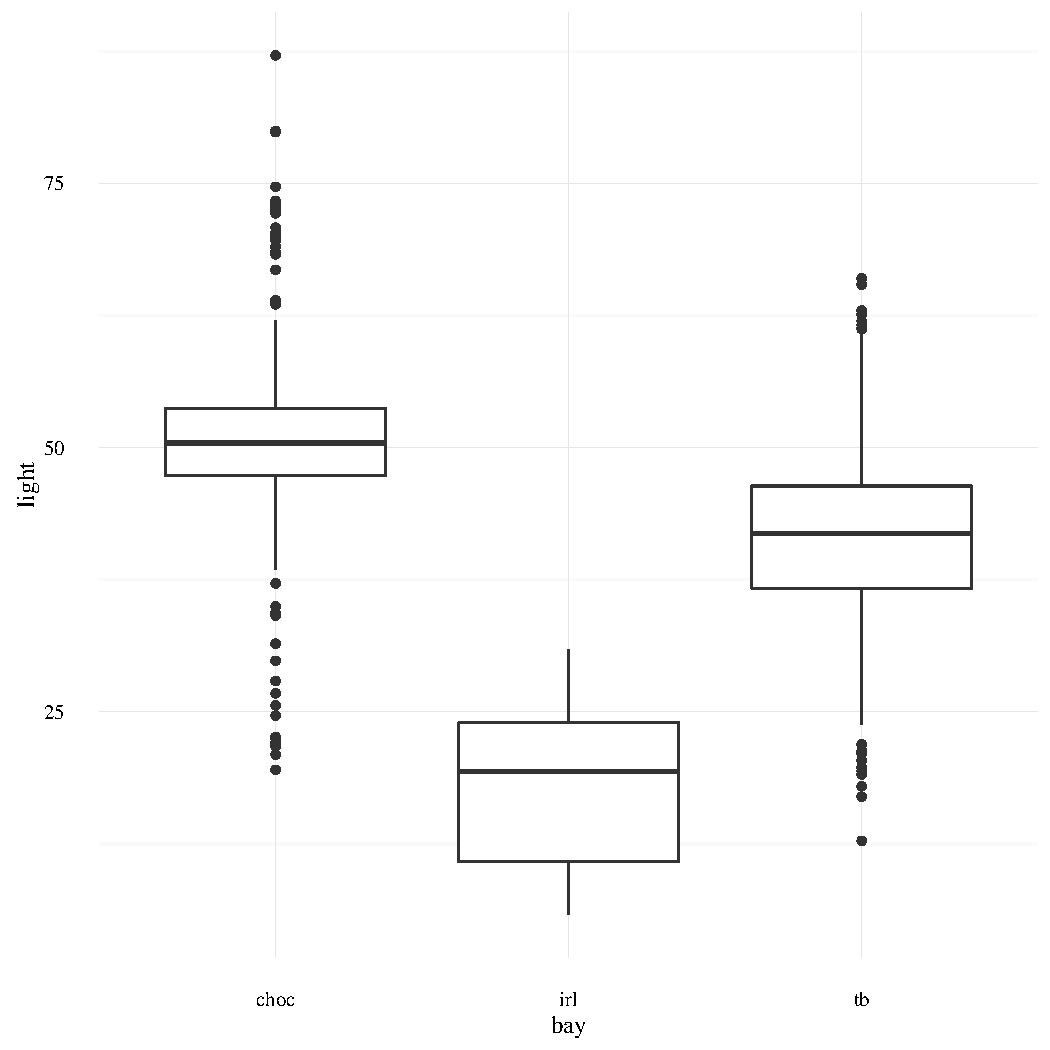
\includegraphics[width=\maxwidth]{fig/unnamed-chunk-3-1} 

}



\end{knitrout}

\begin{knitrout}
\definecolor{shadecolor}{rgb}{0.969, 0.969, 0.969}\color{fgcolor}\begin{kframe}
\begin{alltt}
\hlkwd{summary}\hlstd{(zm1)}
\end{alltt}
\begin{verbatim}
## Linear mixed-effects model fit by REML
##  Data: all_light 
##         AIC       BIC   logLik
##   -87.99629 -59.64608 49.99814
## 
## Random effects:
##  Formula: ~1 | bay
##         (Intercept)  Residual
## StdDev:  0.04474165 0.2800867
## 
## Correlation Structure: Gaussian spatial correlation
##  Formula: ~Latitude + Longitude | bay 
##  Parameter estimate(s):
##       range 
## 0.007992795 
## Fixed effects: z_c_all ~ 0 + bay 
##            Value  Std.Error DF  t-value p-value
## baychoc 2.124354 0.05637388  0 37.68330     NaN
## bayirl  1.073833 0.06374245  0 16.84643     NaN
## baytb   1.199982 0.04764828  0 25.18416     NaN
##  Correlation: 
##        baychc bayirl
## bayirl 0            
## baytb  0      0     
## 
## Standardized Within-Group Residuals:
##        Min         Q1        Med         Q3        Max 
## -5.6196257 -0.5367480  0.2614813  0.9666520  7.3331159 
## 
## Number of Observations: 836
## Number of Groups: 3
\end{verbatim}
\begin{alltt}
\hlkwd{summary}\hlstd{(lm1)}
\end{alltt}
\begin{verbatim}
## Linear mixed-effects model fit by REML
##  Data: all_light 
##        AIC      BIC    logLik
##   5680.798 5709.149 -2834.399
## 
## Random effects:
##  Formula: ~1 | bay
##         (Intercept) Residual
## StdDev:    1.335232  8.35838
## 
## Correlation Structure: Gaussian spatial correlation
##  Formula: ~Latitude + Longitude | bay 
##  Parameter estimate(s):
##       range 
## 0.007154898 
## Fixed effects: light ~ 0 + bay 
##            Value Std.Error DF  t-value p-value
## baychoc 51.19770  1.640932  0 31.20037     NaN
## bayirl  17.83239  1.889493  0  9.43766     NaN
## baytb   41.65458  1.408418  0 29.57544     NaN
##  Correlation: 
##        baychc bayirl
## bayirl 0            
## baytb  0      0     
## 
## Standardized Within-Group Residuals:
##          Min           Q1          Med           Q3          Max 
## -3.791201263 -0.554951340 -0.005255754  0.506392145  4.296715152 
## 
## Number of Observations: 836
## Number of Groups: 3
\end{verbatim}
\end{kframe}
\end{knitrout}

\begin{kframe}
\begin{alltt}
\hlkwd{stargazer}\hlstd{(znl, zm1, zm2, lnl, lm1, lm2,}
  \hlkwc{title} \hlstd{=} \hlstr{'Inter-bay differences for median depth of colonization and light requirements. Null models do not include a grouped correlation structure. Gaussian models with and without nuggets for the spatial correlation structures are also shown.'}\hlstd{,}
  \hlkwc{column.labels} \hlstd{=} \hlkwd{c}\hlstd{(}\hlstr{'null'}\hlstd{,} \hlstr{'Gaus'}\hlstd{,} \hlstr{'Gaus, nug'}\hlstd{,} \hlstr{'null'}\hlstd{,} \hlstr{'Gaus'}\hlstd{,} \hlstr{'Gaus, nug'}\hlstd{),}
  \hlkwc{model.numbers} \hlstd{= F}
  \hlstd{)}
\end{alltt}
\end{kframe}
% Table created by stargazer v.5.2 by Marek Hlavac, Harvard University. E-mail: hlavac at fas.harvard.edu
% Date and time: Sun, May 22, 2016 - 11:26:12 AM
\begin{table}[!htbp] \centering 
  \caption{Inter-bay differences for median depth of colonization and light requirements. Null models do not include a grouped correlation structure. Gaussian models with and without nuggets for the spatial correlation structures are also shown.} 
  \label{} 
\begin{tabular}{@{\extracolsep{5pt}}lcccccc} 
\\[-1.8ex]\hline 
\hline \\[-1.8ex] 
 & \multicolumn{6}{c}{\textit{Dependent variable:}} \\ 
\cline{2-7} 
\\[-1.8ex] & \multicolumn{3}{c}{z\_c\_all} & \multicolumn{3}{c}{light} \\ 
 & null & Gaus & Gaus, nug & null & Gaus & Gaus, nug \\ 
\hline \\[-1.8ex] 
 baychoc & 2.242 & 2.124 & 2.021 & 50.758 & 51.198 & 48.077 \\ 
  & (0.059) & (0.056) & (0.110) & (1.528) & (1.641) & (3.012) \\ 
  & & & & & & \\ 
 bayirl & 1.054 & 1.074 & 1.101 & 17.932 & 17.832 & 17.664 \\ 
  & (0.075) & (0.064) & (0.096) & (1.946) & (1.889) & (2.591) \\ 
  & & & & & & \\ 
 baytb & 1.210 & 1.200 & 1.163 & 41.577 & 41.655 & 42.062 \\ 
  & (0.057) & (0.048) & (0.081) & (1.474) & (1.408) & (2.202) \\ 
  & & & & & & \\ 
\hline \\[-1.8ex] 
Observations & 836 & 836 & 836 & 836 & 836 & 836 \\ 
Log Likelihood & $-$303.580 & 49.998 & 537.481 & $-$3,011.239 & $-$2,834.399 & $-$2,542.856 \\ 
Akaike Inf. Crit. & 617.160 & $-$87.996 & $-$1,060.961 & 6,032.477 & 5,680.798 & 5,099.712 \\ 
Bayesian Inf. Crit. & 640.785 & $-$59.646 & $-$1,027.886 & 6,056.103 & 5,709.149 & 5,132.787 \\ 
\hline 
\hline \\[-1.8ex] 
\textit{Note:}  & \multicolumn{6}{r}{$^{*}$p$<$0.1; $^{**}$p$<$0.05; $^{***}$p$<$0.01} \\ 
\end{tabular} 
\end{table} 


\begin{knitrout}
\definecolor{shadecolor}{rgb}{0.969, 0.969, 0.969}\color{fgcolor}\begin{kframe}
\begin{alltt}
\hlkwd{library}\hlstd{(multcomp)}
\hlkwd{summary}\hlstd{(}\hlkwd{glht}\hlstd{(zm1,} \hlkwc{linfct} \hlstd{=} \hlkwd{mcp}\hlstd{(}\hlkwc{bay} \hlstd{=} \hlstr{'Tukey'}\hlstd{)))}
\end{alltt}
\begin{verbatim}
## 
## 	 Simultaneous Tests for General Linear Hypotheses
## 
## Multiple Comparisons of Means: Tukey Contrasts
## 
## 
## Fit: lme.formula(fixed = z_c_all ~ 0 + bay, data = all_light, random = ~1 | 
##     bay, correlation = corGaus(form = ~Latitude + Longitude | 
##     bay, nugget = FALSE))
## 
## Linear Hypotheses:
##                 Estimate Std. Error z value Pr(>|z|)    
## irl - choc == 0 -1.05052    0.08509 -12.345   <1e-04 ***
## tb - choc == 0  -0.92437    0.07381 -12.523   <1e-04 ***
## tb - irl == 0    0.12615    0.07958   1.585    0.251    
## ---
## Signif. codes:  0 '***' 0.001 '**' 0.01 '*' 0.05 '.' 0.1 ' ' 1
## (Adjusted p values reported -- single-step method)
\end{verbatim}
\begin{alltt}
\hlkwd{summary}\hlstd{(}\hlkwd{glht}\hlstd{(zm2,} \hlkwc{linfct} \hlstd{=} \hlkwd{mcp}\hlstd{(}\hlkwc{bay} \hlstd{=} \hlstr{'Tukey'}\hlstd{)))}
\end{alltt}
\begin{verbatim}
## 
## 	 Simultaneous Tests for General Linear Hypotheses
## 
## Multiple Comparisons of Means: Tukey Contrasts
## 
## 
## Fit: lme.formula(fixed = z_c_all ~ 0 + bay, data = all_light, random = ~1 | 
##     bay, correlation = corGaus(form = ~Latitude + Longitude | 
##     bay, nugget = TRUE))
## 
## Linear Hypotheses:
##                 Estimate Std. Error z value Pr(>|z|)    
## irl - choc == 0 -0.91965    0.14626  -6.288   <1e-05 ***
## tb - choc == 0  -0.85789    0.13672  -6.275   <1e-05 ***
## tb - irl == 0    0.06176    0.12606   0.490    0.876    
## ---
## Signif. codes:  0 '***' 0.001 '**' 0.01 '*' 0.05 '.' 0.1 ' ' 1
## (Adjusted p values reported -- single-step method)
\end{verbatim}
\begin{alltt}
\hlkwd{summary}\hlstd{(}\hlkwd{glht}\hlstd{(lm1,} \hlkwc{linfct} \hlstd{=} \hlkwd{mcp}\hlstd{(}\hlkwc{bay} \hlstd{=} \hlstr{'Tukey'}\hlstd{)))}
\end{alltt}
\begin{verbatim}
## 
## 	 Simultaneous Tests for General Linear Hypotheses
## 
## Multiple Comparisons of Means: Tukey Contrasts
## 
## 
## Fit: lme.formula(fixed = light ~ 0 + bay, data = all_light, random = ~1 | 
##     bay, correlation = corGaus(form = ~Latitude + Longitude | 
##     bay, nugget = FALSE))
## 
## Linear Hypotheses:
##                 Estimate Std. Error z value Pr(>|z|)    
## irl - choc == 0  -33.365      2.503 -13.332   <1e-04 ***
## tb - choc == 0    -9.543      2.162  -4.413   <1e-04 ***
## tb - irl == 0     23.822      2.357  10.108   <1e-04 ***
## ---
## Signif. codes:  0 '***' 0.001 '**' 0.01 '*' 0.05 '.' 0.1 ' ' 1
## (Adjusted p values reported -- single-step method)
\end{verbatim}
\begin{alltt}
\hlkwd{summary}\hlstd{(}\hlkwd{glht}\hlstd{(lm2,} \hlkwc{linfct} \hlstd{=} \hlkwd{mcp}\hlstd{(}\hlkwc{bay} \hlstd{=} \hlstr{'Tukey'}\hlstd{)))}
\end{alltt}
\begin{verbatim}
## 
## 	 Simultaneous Tests for General Linear Hypotheses
## 
## Multiple Comparisons of Means: Tukey Contrasts
## 
## 
## Fit: lme.formula(fixed = light ~ 0 + bay, data = all_light, random = ~1 | 
##     bay, correlation = corGaus(form = ~Latitude + Longitude | 
##     bay, nugget = TRUE))
## 
## Linear Hypotheses:
##                 Estimate Std. Error z value Pr(>|z|)    
## irl - choc == 0  -30.412      3.973  -7.654   <1e-04 ***
## tb - choc == 0    -6.014      3.731  -1.612    0.239    
## tb - irl == 0     24.398      3.400   7.175   <1e-04 ***
## ---
## Signif. codes:  0 '***' 0.001 '**' 0.01 '*' 0.05 '.' 0.1 ' ' 1
## (Adjusted p values reported -- single-step method)
\end{verbatim}
\end{kframe}
\end{knitrout}

\end{document}
